% !TEX root = ../CA_book.tex

\section*{4장 - 연습문제 풀이}

\subsection*{연습문제 \ref{ex-4-1}}

$\Sum_{n=1}^\infty a_n$이 수렴하면,
$\Sum_{n=1}^\infty \Re(a_n)$과 $\Sum_{n=1}^\infty \Im(a_n)$도 각각 수렴한다.
따라서 $\Lim_{n\to\infty} \Re(a_n) = 0$이고, $\Lim_{n\to\infty} \Im(a_n) = 0$이다.
이로부터 $\Lim_{n\to\infty} a_n = 0$이다.

\subsection*{연습문제 \ref{ex-4-2}}

$\Sum_{n=1}^\infty |a_n|$이 수렴한다고 하자.
모든 $ n\in \mathbb N$에 대하여
$\Re(a_n) \le |a_n|$, $\Im(a_n) \le |a_n|$이므로
비교판정법에 의해
\[
\Sum_{n=1}^\infty \Re(a_n), \quad \Sum_{n=1}^\infty \Im(a_n)
\]
이 수렴한다.
따라서 $\Sum_{n=1}^\infty a_n$도 수렴한다.

\subsection*{연습문제 \ref{ex-4-3}}

$s_n:= 1+z+\cdots + z^{n-1}+z^n$이라 하면,
$z s_n = z + z^2 + \cdots + z^n + z^{n+1}$이므로
$(1-z)s_n = 1- z^{n+1}$이다.
$|z|<1$에서  $z\ne1$이므로
\begin{equation}\label{eq-5-21}
s_n = 1+z+\cdots + z^{n-1}+z^n = \dfrac{1-z^{n+1}}{1-z}.
\end{equation}
따라서
\[
\Lim_{n\to\infty} s_n = \lim_{n\to\infty}\dfrac{1-z^{n+1}}{1-z}
= \dfrac{1-0}{1-z} = \dfrac1{1-z}
\]
이므로 $\Sum_{n=0}^\infty z^n$이 수렴하고
$\Sum_{n=0}^\infty z^n = \Lim_{n\to\infty} s_n = \dfrac1{1-z}$이다. \\[1ex]
(이 증명을 위해 $|z|<1$에서
\[
\lim_{n\to\infty} z^{n+1} = 0
\]
을 이용하였다.  이 결과는
$r:=|z|<1$이므로, $|z^{n+1} -0| = |z|^{n+1} \stackrel{n\to\infty}{\longrightarrow }0$으로부터
얻어진다.)

\subsection*{연습문제 \ref{ex-4-4}}

자연수 $n\in\mathbb N$에 대하여 
$s_n:= 1+2z + 3z^2 + \cdots + (n-1)z^{n-2} + nz^{n-1}$이라 하자.
그러면 $zs_n = z + 2z^2 + \cdots + (n-1)z^{n-1} + nz^n$이다.
따라서
\[
(1-z)s_n= 1 + z + z^2 + \cdots + z^{n-1} - nz^n
= \dfrac{1-z^n}{1-z}  - nz^n.
\]
따라서
\[
s_n = \dfrac{1-z^n}{(1-z)^2}  - \dfrac{nz^n}{1-z}.
\]
(이 결과는 식 \eqref{eq-5-21}의 양변을 $z$에 대하여 미분해서 얻을 수도 있다.)

$r:=|z|$ ($0\le r < 1$)이라 하면,
\[
r = \dfrac1{1+h}
\]
여기서 $h:=\dfrac1r-1>0$이다.
\[
(1+h)^n = 1 + {n\choose 1}h + {n \choose 2}h^2 + \cdots
+ {n \choose n}h^n \ge {n \choose 2}h^2 = \dfrac{n\cdot(n-1)}2 \cdot h^2
\]
에서
\[
0\le nr^n = \dfrac n{(1+h)^n} \le n \cdot \dfrac2{n\cdot(n-1)\cdot h^2}
= \dfrac 2{(n-1)\cdot h^2}
\]
이므로
조임정리(Sandwitch theorem)에 의하여 $\Lim_{n\to\infty} nr^n = 0$이다.
결론적으로,
\[
\Lim_{n\to\infty}  s_n = \Lim_{n\to\infty} \left( \dfrac{1-z^n}{(1-z)^2}
- \dfrac{nz^n}{1-z} \right)
= \dfrac{1-0}{(1-z)^2} - \dfrac0{1-z} = \dfrac1{(1-z)^2}.
\]

\subsection*{연습문제 \ref{ex-4-5}}

\begin{align*}
\left| \dfrac1{n^s} \right| &= \left| \dfrac1{\exp(s\cdot \Log(n))} \right|
= \left| \dfrac1{\exp(s\cdot\log n)}\right| \\
&= \dfrac1{e^{\Re(s\cdot \log n)}} = \dfrac1{e^{(\log n)\cdot(\Re(s))}}
= \dfrac1{(e^{\log n})^{\Re(s)}} = \dfrac1{n^{\Re(s)}}.
\end{align*}

$p>1$\,일 때 $\Sum_{n=1}^\infty \dfrac1{n^p}$이 수렴함을 이용하면,
$\Re(s)>1$에 대하여
\[
\sum_{n=1}^\infty \dfrac1{n^{\Re(s)}}
\]
가 수렴한다. 따라서  $\Re(s)>1$인 영역에서
\[
\sum_{n=1}^\infty \dfrac1{n^{s}}
\]
은 절대수렴하므로, 당연히 수렴한다.

\subsection*{연습문제 \ref{ex-4-6}}

$L\ne0$이라고 하자.
$|z|< 1/L$인 모든 $z$에 대하여, 
$N$이 충분히 클 때 $n>N$이면
$\sqrt[n]{|c_nz^n|}  = \sqrt[n]{|c_n|}|z| \le q <1$를 만족하는 $q<1$가 존재한다. 
이 결과는 $\sqrt[n]{|c_n|}|z| \xrightarrow{n\to\infty} L|z|<1$로부터 얻어진 것이다.
(예를 들어 $q=(L|z|+1)/2 <1$로 잡으면 된다.)

$L=0$이면, 
임의의(고정된) $z\in \mathbb C$에 대하여
$n>N$이면 $\sqrt[n]{|c_nz^n|} = \sqrt[n]{|c_n|}|z| \le q < 1$을 항상 만족하는 $q<1$가 존재한다.
이 결과는  $\sqrt[n]{|c_n|}|z| \xrightarrow{n\to\infty} 0|z|=0<1$로부터 얻어진다.
(예를 들어 $q=1/2<1$로 잡으면 된다.)
근판정법(root test)\footnote{
역주:
급수 $\Sum a_n$에 대하여
극한 $L = \Lim_{n\to\infty} \sqrt[n]{|a_n|}$이 존재할 때,
$L<1$이면 급수가 수렴하고
$L>1$이면 급수가 발산한다.
}을 쓰면 제곱급수가 수렴함을 알 수 있다.

한편, $L\ne0$이고 $|z|>1/L$인 경우를 생각하면
$N$이 충분히 클 때 모든 $n>N$에 대하여
$\sqrt[n]{|c_nz^n|}  = \sqrt[n]{|c_n|}|z| >1$가 성립한다.
이 결과는  $\sqrt[n]{|c_n|}|z| \xrightarrow{n\to\infty} L|z|>1$로부터 얻어진다.
다시 근판정법을 쓰면 이 경우 제곱급수가 발산함을 알 수 있다.

\subsection*{연습문제 \ref{ex-4-7}}

$z=0$일 때 급수가 $0$으로 수렴함은 자명하다.
$z\ne 0$라고 가정하자. 그러면, $N>1/|z|$인 
$N\in\mathbb N$를 선택할 수 있다.
$n>N$에 대하여 $|nz|>N|z|>1$이고
$|n^nz^n -0| = |nz|^n >1^n = 1$이므로
\[
\neg \left( \lim_{n\to\infty} n^n z^n = 0 \right).
\]
따라서 $z\ne0$이면, $\Sum_{n=1}^\infty n^n z^n$은 발산한다.

\subsection*{연습문제 \ref{ex-4-8}}

$\Lim_{n\to\infty} \sqrt[n]{\dfrac1{n^n}} = \Lim_{n\to\infty} \dfrac1n = 0$이므로
\[
\sum_{n\to\infty} \dfrac{z^n}{n^n}
\]
의 수렴 반지름은 무한대이고 이 제곱급수는 모든 $z\in\mathbb C$에 대하여 수렴한다.

\subsection*{연습문제 \ref{ex-4-9}}

\begin{itemize}
\item[(1)] 
\[
\lim_{n\to\infty} \left| \dfrac{\dfrac{(-1)^{n+1}}{n+1}}{\dfrac{(-1)^n}n} \right|
= \lim_{n\to\infty} \dfrac n{n+1} = 1
\]
이므로 $\Sum_{n=1}^\infty \dfrac{(-1)^n}n z^n$의 수렴 반지름은 $1$이다.

\item[(2)] 
\[
\lim_{n\to\infty} \left| \dfrac{(n+1)^{2012}}{n^{2012}} \right|
= \lim_{n\to\infty} \left( 1+ \dfrac1{n} \right)^{2012} = 1
\]
이므로 $\Sum_{n=1}^\infty n^ {2012} z^n$의 수렴 반지름은 $1$이다.

\item[(3)] 
\[
\lim_{n\to\infty} \left| \dfrac{\dfrac{1}{(n+1)!}}{\dfrac1{n!}} \right|
= \lim_{n\to\infty} \dfrac1{n+1} = 0
\]
이므로 $\Sum_{n=1}^\infty \dfrac1{n!}z^n$의 수렴 반지름은 무한대이다.
\end{itemize}

\subsection*{연습문제 \ref{ex-4-10}}

$|z|<1$에 대하여
\[
f(z):= 1+2z+ 3z^2 + 4z^3 + \cdots = \dfrac 1{(1-z)^2}
\]
이므로 
\[
zf(z) = g(z) := z + 2z^2 + 3z^3 + 4z^4 + \cdots = \dfrac z{(1-z)^2}
\]
임을 알고 있다.
따라서 $g(z):= z+2z^2+3z^3 + 4z^4 + \cdots$이 $|z|<1$에서 수렴하므로
$g$는 원판 $|z|<1$에서 복소해석함수이고
$g'(z) = 1 + 2^2z + 3^2z^2 + 4^2z^3 + \cdots$이다.
한편,
\[
g(z) = zf(z) = \dfrac z{(1-z)^2}
\]
이므로
\[
g'(z) = \dfrac d{dz} \left( \dfrac z{(1-z)^2} \right)
= 1\cdot \dfrac1{(1-z)^2} + z\cdot\dfrac 2{(1-z)^3}
= \dfrac{1-z+2z}{(1-z)^3} = \dfrac{1+z}{(1-z)^3}
\]
이 원하는 결과이다.

\subsection*{연습문제 \ref{ex-4-11}}

\begin{itemize}
\item[(1)] 거짓. \\
예를 들면, $\left\{ z\in\mathbb C\,:\, \Sum_{n=1}^\infty \dfrac{z^n}{n^2} \text{\,가 수렴한다.} \right\}
= \left\{ z\in\mathbb C\,:\, |z|\le 1\right\}$는 ``닫힌''영역이다.
\item[(2)] 참.
\item[(3)] 거짓.  \\
예를 들면, $\Sum_{n=1}^\infty \dfrac{(-1)^n}n z^n$은 $z=1$에서 수렴하지만
$z=-1$에서는 발산한다.
\item[(4)] 거짓. (3)의 예를 참고하라.
\item[(5)] 참. (3)의 예를 참고하라.
\item[(6)] 참. 예를 들면, $\Sum_{n=1}^\infty \dfrac{z^n}{n^2}$.
\item[(7)] 참. 수렴 반지름은 $1$보다 작거나 같고, $|1+i| = \sqrt{2} >1$이다.
\end{itemize}

\subsection*{연습문제 \ref{ex-4-12}}

$\sin 0 = 0$, $\cos 0 =1$이고,
\[
\dfrac{d^{2n}}{dz^{2n}} \sin z = (-1)^n \sin z,
\quad
\dfrac{d^{2n+1}}{dz^{2n+1}} \sin z = (-1)^n \cos z
\]
이므로 
\[
\sin z = \sum_{n=0}^\infty \dfrac1{n!} \left(\dfrac{d^n}{dz^n} \sin z \right)\Big|_{z=0}
= z - \dfrac{z^3}{3!} + \dfrac{z^5}{5!} - \cdots
\]
유사한 방법으로 $\cos z = 1 - \dfrac{z^2}{2!} + \dfrac{z^4}{4!} - \cdots$도 얻을 수 있다.

전혀 다른 방법으로 구해보면,
\[
\cos z = \dfrac{\exp(iz)  + \exp(-iz)}2 
= \dfrac12 \left( \sum_{n=0}^\infty \dfrac1{n!}i^nz^n 
+ \sum_{n=0}^\infty \dfrac1{n!}(-1)^ni^nz^n \right)
\]
이므로, $i^{2n} = (-1)^n$을 이용하면,
\begin{align*}
\cos z &= \dfrac12 \left(
1+ iz - \dfrac{z^2}{2!} - \dfrac{iz^3}{3!} + \dfrac{z^4}{4!} \right.
+ \dfrac{iz^5}{5!} - \dfrac{z^6}{6!}  + \cdots \\
&\qquad\left. +1 - iz - \dfrac{z^2}{2!} + \dfrac{iz^3}{3!} + \dfrac{z^4}{4!} 
- \dfrac{iz^5}{5!} - \dfrac{z^6}{6!}  + \cdots \right) \\
&= 1 - \dfrac1{2!}z^2 + \dfrac1{4!}z^4 - \dfrac1{6!}z^6 + \cdots.
\end{align*}

\subsection*{연습문제 \ref{ex-4-13}}

$p(z) = z^6 -z^4 +z^2 -1$, $z\in \mathbb C$라 하면,
\begin{align*}
& p'(z) = 6z^5 - 4z^3 +2z, \\
& p''(z) = 30z^4 -12z^2 + 2, \\
&p'''(z) = 120z^3 - 24z, \\
&p^{(4)}(z) = 360z^2 - 24, \\
&p^{(5)}(z) = 720z, \\
&p^{(6)}(z) = 720, \\
&p^{(7)}(z) = p^{(8)}(z) = \cdots = 0
\end{align*}
이므로,
\begin{align*}
&p(1) = 1-1+1-1 = 0, \\
&\dfrac{p'(1)}{1!} = 6 - 4 + 2 = 4, \\
&\dfrac{p''(1)}{2!} = \dfrac{30-12+2}{2} = 10, \\
&\dfrac{p'''(1)}{3!} = \dfrac{120-24}{6} = 16, \\
&\dfrac{p^{(4)}(1)}{4!} = \dfrac{360-24}{24} = 14, \\
&\dfrac{p^{(5)}(1)}{5!} = \dfrac{720}{120} = 6, \\
&\dfrac{p^{(6)}(1)}{6!} = \dfrac{720}{720} = 1.
\end{align*}
따라서 모든 $z\in\mathbb C$에 대하여,
\begin{align*}
z^6&-z^4+z^2-1 \\
&= p(1) + \dfrac{p'(1)}{1!}(z-1) + \cdots + \dfrac{p^{(6)}(1)}{6!}(z-1)^6 + 0 \\
&= 4(z-1) + 10(z-1)^2 + 16(z-1)^3 + 14(z-1)^4 + 6(z-1)^5 + (z-1)^6.
\end{align*}

\subsection*{연습문제 \ref{ex-4-14}}

\begin{itemize}
\item[(1)] 
단순연결 영역 $\mathbb C$에서
$z\mapsto \exp(z^2)$은 부정적분을 가지며, 이를 $g$라 하면
\[
f(z) = \int_{\gamma_{0z}} \exp(\zeta^2) d\zeta 
= \int_{\gamma_{0z}} g'(\zeta) d\zeta = g(z) - g(0).
\]
따라서 $f'(z) = g'(z) = \exp(z^2) = \Sum_{n=0}^\infty \dfrac1{n!}z^{2n}$.
\[
\dfrac1{(2n)!} \dfrac{d^{2n}}{dz^{2n}}f'(z) \Big|_{z=0} = \dfrac1{n!}, 
\quad
\dfrac1{(2n+1)!} \dfrac{d^{2n+1}}{dz^{2n+1}}f'(z) \Big|_{z=0} = 0
\]
이므로
$f^{(2n+1)}(0) = \dfrac{(2n)!}{n!}$, $f^{(2n+2)}(0) = 0$이고, $f(0)=0$이다.
따라서,
\[
f(z) = \sum_{n=0}^\infty \dfrac{f^{(n)}(0)}{n!} z^n 
= \sum_{n=0}^\infty \dfrac{f^{(2n+1)}(0)}{(2n+1)!} z^{2n+1}
= \sum_{n=0}^\infty \dfrac1{(2n+1)(n!)} z^{2n+1}.
\]
\item[(2)] 
$|z|<1$에 대하여,
\[
\dfrac1{z+1} = 1 - z + z^2 - z^3 + z^4 - \cdots
\]
이고 제곱급수는 수렴하는 영역에서 복소해석함수이고 항별미분이 가능하기 때문에
$|z|<1$에서
\[
- \dfrac1{(z+1)^2} = \dfrac d{dz}\dfrac1{z+1} = - 1 + 2z - 3z^2 + 4z^3 - \cdots
\]
양변에 $-z^2$을 곱하면, $|z|<1$에서
\[
 \dfrac{z^2}{(z+1)^2} =z^2 - 2z^3 + 3z^4 - \cdots
= \sum_{n=2}^\infty (-1)^n\cdot (n-1)\cdot z^n
\]
이므로 $c_0=c_1=0$이고, $c_n =(-1)^n\cdot(n-1)$ ($n\ge2$)이다.
\end{itemize}

\subsection*{연습문제 \ref{ex-4-15}}

$z\in\mathbb C$에 대하여 $R>|z|$을 잡으면,
\begin{align*}
|f^{(n+1)}(z)| &\le \dfrac{(n+1)!}{R^{n+1}}\cdot \max_{|z|\le R} |f(z)| \\
&\le \dfrac{(n+1)!}{R^{n+1}}\cdot \max_{|z|\le R} M\cdot |z|^n 
= \dfrac{(n+1)!}{R^{n+1}}\cdot M\cdot R^n = \dfrac{(n+1)!M}R.
\end{align*}
$R>|z|$의 선택을 임의로 크게 할 수 있기 때문에
$f^{(n+1)}(z) = 0$이다.
어떤 $z\in \mathbb C$을 선택해도 같은 결과를 얻기 때문에
$\mathbb C$ 전체에서 $f^{(n+1)} \equiv 0$이다.
테일러 정리에 의해,  모든 $z\in \mathbb C$에 대하여
\[
f(z) = \sum_{k=0}^\infty \dfrac{f^{(k)}(0)}{k!} (z-0)^k
= \sum_{k=0}^n \dfrac{f^{(k)}(0)}{k!} z^k.
\]
$f^{(n+1)}(0) = f^{(n+2)}(0) = f^{(n+3)}(0) = \cdots 0$이므로
$f$는 기껏해야 $n$차 다항식이다.

조건에서 $n=0$이면, $f$는 유계인 전해석 함수이며
위의 결론에서 $f$는 상수함수이다 ($0$차 다항식).
따라서 특별히 $n=0$인 경우는 리우비유 정리와 일치한다.

\subsection*{연습문제 \ref{ex-4-16}}

코시 적분공식에 의해
\begin{align*}
\dfrac{2013!}{2\pi i}  \int_C \dfrac{\sin z}{z^{2013}}dz
&= \dfrac{d^{2012}}{dz^{2012}} \sin z \Big|_{z=0} \\
&= (-1)^{2012/2} \sin z\Big|_{z=0} \\
&=0
\end{align*}
이므로  $ \dint_C \dfrac{\sin z}{z^{2013}}dz=0$.

\subsection*{연습문제 \ref{ex-4-17}}

$z_0$에서 $g$의 연속성에 의해
$|z-z_0|<\delta$에서 $g(z)\ne0$가 되도록 $R$보다 작은 $\delta>0$를 잡을 수 있다.
$f(z_0)=0$이고 $f(z) = (z-z_0)^mg(z)$ ($|z-z_0|<R$)이므로
$0<|z-z_0|<\delta$에서  $f(z)\ne0$이다.
근의 분류 정리에 의하여
$f$는 $z_0$에서 $\tilde m\in \mathbb N$ 중근을 갖고
$\tilde g(z_0)\ne0$인 복소해석함수 $\tilde g$가 존재한다.
이제 $|z-z_0|<R$에서
$(z-z_0)^{\tilde m} \tilde g(z) = (z-z_0)^m g(z)$가 성립한다.
$\tilde m = m$임을 증명해보자.
$\tilde m >m$이라면,
\[
0\ne g(z_0) = \lim_{z\to z_0} g(z) = \lim_{z\to z_0} (z-z_0)^{\tilde m - m}\tilde g(z_0) 
= 0\cdot \tilde g(z_0)= 0
\]
가 되어 모순에 도달한다. 반대로 $m>\tilde m$이면,
\[
0\ne \tilde g(z_0) = \lim_{z\to z_0} \tilde g(z) = \lim_{z\to z_0} (z-z_0)^{m - \tilde m} g(z_0) 
= 0\cdot g(z_0)= 0
\]
로 모순이다.
따라서, $m= \tilde m$이 되고, $z_0$는 $m$ 중근이다.

\subsection*{연습문제 \ref{ex-4-18}}

\begin{itemize}
\item[(1)] 
\[f(z) = (1+z^2)^4 = ((z-i)(z+i))^4
= (z-i)^4(z+i)^4
\]
이므로 $g(z):= (z+i)^4$이라 하면
$g$는 전해석 함수이고 $g(i) = (2i)^4 = 16\ne 0$이고
$f(z) = (z-i)^4 g(z)$이다. 
따라서 $i$는 $f$의 $4$중근이다.
\item[(2)] 
\begin{align*}
f(2n\pi i) &= 1 - 1 = 0, \\
f'(2n\pi i) &= \exp z \Big|_{z=2n\pi i} = 1 \ne 0
\end{align*}
이므로  $f$의 근 $2n\pi i$의 차수는 $1$이다.
\item[(3)] $f(0)  = 1 - 1 + \dfrac12(0)^2 = 0$이고
\begin{align*}
f(z) &= \cos z - 1 + \dfrac12(\sin z)^2 = \cos z - 1 + \dfrac12 \cdot \dfrac{(1-\cos(2z))}2 \\
&= \cos z - \dfrac34 - \dfrac14\cos(2z) \\
&= \left( 1 - \dfrac{z^2}{2!} + \dfrac{z^4}{4!} - \dfrac{z^6}{6!} + \cdots \right)- \dfrac 34 \\
& \qquad -\dfrac14\left( 1 - \dfrac{4z^2}{2!} + \dfrac{16z^4}{4!} 
- \dfrac{2^6z^6}{6!} + \cdots \right) \\
&= \underbrace{\left(1-\dfrac34-\dfrac14\right)}_{0}
+ \underbrace{\left(-\dfrac1{2!} +\dfrac14\cdot\dfrac 4{2!}\right)}_{0} z^2
+ \underbrace{\left(\dfrac1{4!} - \dfrac14\cdot\dfrac {16}{4!}\right)}_{\ne 0} z^4 + \cdots
\end{align*}
이므로 근 $z_0$의 차수는 $4$이다.
\end{itemize}

\subsection*{연습문제 \ref{ex-4-19}}

원판에서 $z_0$와 다른 점 $z$를 잡으면 $f(z)\ne0$이다.
근의 분류 정리에서 $f(z)=(z-z_0)g(z)$로 쓸 수 있다.
여기서 $g$는 복소해석함수이고 $g(z_0)\ne0$이다.
\begin{align*}
\dfrac1{2\pi i}\int_\gamma \dfrac{zf'(z)}{f(z)}dz 
&= \dfrac1{2\pi i}\int_\gamma \dfrac{z(1\cdot g(z) + (z-z_0)\cdot g'(z))}{(z-z_0)g(z)}dz  \\
&= \dfrac1{2\pi i}\int_\gamma \dfrac{\dfrac{z(g(z) + (z-z_0)\cdot g'(z))}{g(z)}}{(z-z_0)}dz  \\
&= \dfrac{z(g(z) + (z-z_0)\cdot g'(z_0))}{g(z)}\Big|_{z=z_0} 
\quad\text{(코시 적분공식에 의해)} \\
&= \dfrac{z_0(g(z_0) + 0\cdot g'(z_0))}{g(z_0)} \\
&= z_0.
\end{align*}

\subsection*{연습문제 \ref{ex-4-20}}

근의 분류 정리에 의해 $f(z)=(z-z_0)^m g(z)$로 쓸 수 있고
$g$는 $D$에서 복소해석함수이고 $g(z_0)\ne0$이다.
\[
\left( f(z) \right)^2 = (z-z_0)^{2m} 
\underbrace{ \left( g(z) \right)^2}_{=:G(z)}.
\]
$(f(z_0))^2=0$임은 분명하고 $G$는 $D$에서 복소해석함수로 
$G(z_0) = (g(z_0))^2 \ne 0$이다.
따라서 $z\mapsto (f(z))^2$은 $z_0$에서 $2m$ 중근을 갖는다.
또한,
\begin{align*}
f'(z) &= m(z-z_0)^{m-1} g(z) + (z-z_0)^m g'(z) \\
&= (z-z_0)^{m-1} \underbrace{(mg(z) + (z-z_0)g'(z))}_{=:g_1(z)}
\end{align*}
이므로 $f'(z_0) = (z_0 - z_0)^{m-1}g_1(z_0) \stackrel{(m>1)}{=}
0\cdot g_1(z_0) = 0$.
$g_1$은 복소해석함수이고 
\[
g_1(z_0) = mg(z_0) + 0\cdot g'(z_0) = mg(z_0) + 0 = mg(z_0) \ne 0
\]
이므로 $z_0$는 $f'$의 $m-1$ 중근이다.

\subsection*{연습문제 \ref{ex-4-21}}

함수 $f:\mathbb C \to \mathbb C$를
\[
f(x,y) = x\sin \dfrac1x, \quad (x\ne0)
\]
$f(0,*)=0$으로 정의하자.
그러면 $f$는 $x_0\ne0$인 $(x_0, y_0)$에서 연속임은 자명하다.
모든 $x\ne0$에 대하여
\[
|f(x,y_0) - f(0,y_0)|= \left| x\sin \dfrac1x - 0\right| = |x| \left| \sin \dfrac 1x \right|
\le |x| \cdot 1 = |x-0|
\]
이므로 $f$는 $(0,*)$에서 연속임이 분명하다.
따라서 $f$는 $\mathbb C$의 모든 점에서 연속이다.
정의에서 $0$은 $f$의 근이지만 
\[
f\left( \dfrac1{n\pi}, 0\right) = \dfrac1{n\pi} \sin(n\pi) = 0, \quad n\in\mathbb N
\]
이므로 고립 근은 아니다.
또한, $f$는 $0$을 중심으로 하는 어떤 원판의 내부에서 항등적으로 $0$이 될 수 없다.
왜냐하면, $n\in\mathbb N$에 대하여,
\[
f\left( \dfrac2{(2n+1)\pi}, 0\right) 
= \dfrac2{(2n+1)\pi}\sin\left((2n+1)\dfrac\pi2 \right) 
=\dfrac2{(2n+1)\pi}(-1)^n \ne0
\]
이기 때문이다.

\subsection*{연습문제 \ref{ex-4-22}}

실수 $x_1, x_2 \in\mathbb R$에 대하여
\begin{equation}\label{eq-5-22}
\cos (x_1 + x_2) = (\cos x_1)(\cos x_2) - (\sin x_1)(\sin x_2)
\end{equation}
가 성립함을 알고 있다.
$x\in \mathbb R$을 고정하고 전해석 함수 $f$를 다음과 같이 정의하자.
\[
f(z):= \cos(z+x) - \left( (\cos z)(\cos x) - (\sin z)(\sin x) \right),
z\in\mathbb C.
\]
그러면 $y\in\mathbb R$에 대하여 $f(y)=0$이다.
식 \eqref{eq-5-22}\와 항등정리로부터
모든 $z\in\mathbb C$에서 $f(z)=0$이다.
즉,
\begin{equation}\label{eq-5-23}
\cos (z + x) = (\cos z)(\cos x) - (\sin z)(\sin x),\quad z\in\mathbb C.
\end{equation}
$x\in\mathbb R$의 선택을 임의로 할 수 있기 때문에
식 \eqref{eq-5-23}\은  모든 $x\in\mathbb R$에 대하여 성립한다.
다음 단계로, $z\in\mathbb C$를 고정하여
전해석 함수 $g$를 만들자.
\[
g(w):= \cos(z+w) - \left( (\cos z)(\cos w) - (\sin z)(\sin w) \right), \quad w\in\mathbb C.
\]
그러면 식 \eqref{eq-5-23}에 의하여 
모든 $x\in\mathbb R$에서 $g(x)=0$이다.
항등정리를 다시 적용하면 모든 $w\in\mathbb C$에서 $g(w)=0$을 얻는다.
따라서
\begin{equation}\label{eq-5-24}
\cos (z+w) =  (\cos z)(\cos w) - (\sin z)(\sin w), \quad w\in\mathbb C.
\end{equation}
이 식에서 $z\in\mathbb C$의 선택을 임의로 할 수 있기 때문에,
결론적으로 식 \eqref{eq-5-24}\는 모든 $z\in\mathbb C$(와 모든 $w\in\mathbb C$)에
대하여 성립한다.

\subsection*{연습문제 \ref{ex-4-23}}

$f,g\in\Hol(D)$가
\begin{equation}\label{eq-5-25}
(f\cdot g) = f(z)\cdot g(z) = 0, \quad z\in D
\end{equation}
을 만족한다고 가정하자.
$z_0\in D$에서 $f(z_0)\ne0$라고 가정하자. 그러면
$f$가 연속함수이므로,
$|z-z_0|<\delta$이면 $f(z)\ne0$가 되는 $\delta>0$가 존재한다.
식 \eqref{eq-5-25}\로부터 $|z-z_0|<\delta$에서 
$g(z)=0$이고, 항등정리에 의해 $D$에서 $g\equiv 0$이다.
따라서 $\Hol(D)$는 영인자(zero divisor)를 갖지 않는다.

한편, 연속함수 $C(D)$는 정역(integral domain)이 아닌데
이를 다음과 같이 보일 수 있다.
$z_0\in D$에 대하여
\[
\Delta := \{ z\in D \,:\, |z-z_0| <\delta \} \subset D
\]
인 $\delta >0$를 생각하자.
연속함수 $\varphi: \mathbb R \to \mathbb R$을
\[
\varphi(t) = \begin{cases}
0, & t\le 0, \\
t, & t>0
\end{cases}
\]
이라 정의하고, $z\in D$에 대하여
\begin{align*}
f(z) &:=  \varphi(\Re(z-z_0)), \\
g(z) &:=  \varphi(-\Re(z-z_0))
\end{align*}
라 하면, 
연속함수의 합성이므로 $ f, g\in C(D)$이다.
또한, $\Delta$의 오른쪽 반원에 속하는 모든 $z$에 대하여 $f(z)>0$이므로
연속함수로서 $f\ne0$이다. 같은 방법으로 
$\Delta$의 왼쪽 반원에 속하는 모든 $z$에 대하여 $g(z)>0$이므로
$g\ne0$이다. 그럼에도 불구하고 $f\cdot g=0$이다.

\begin{figure}[h!]
\begin{center}
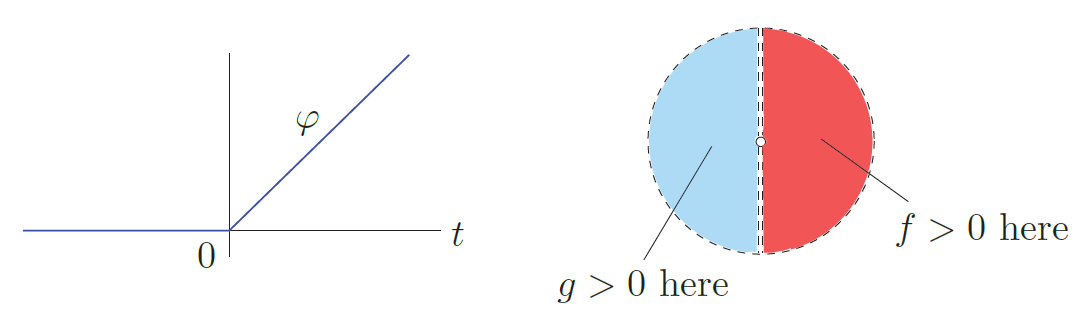
\includegraphics[width=0.8\textwidth]{./Solution/figs/fig-5-21}
\end{center}
\caption{$\varphi$를 이용한 연속함수 $f,g\in C(D)$의 구성
}
\label{fig-5-21}
\end{figure}

\subsection*{연습문제 \ref{ex-4-24}}

\begin{itemize}
\item[(1)]   거짓.
$D=\mathbb C$, $f=\exp$, $g=1$이라 하자.
그러면, 모든 $n\in \mathbb N$에 대하여
$f(2\pi i n) = \exp(2\pi i n) = 1 = g(2\pi i n)$이고,
$f\ne g$이다 (예를 들면, $f(i\pi) = -1 \ne 1 = g(i\pi)$).
\item[(2)] 참.
\item[(3)] 참. 
$\gamma(t) = x(t) +iy(t)$, $t\in[a,b]$라 하자.
$x'(t_0)$ 또는 $y'(t_0)$가 $0$이 아닌 점 $t_0$를 생각하자.
(이런 점이 없다면 두 값이 항상 $0$이므로 $a=b$가 되어 모순이다.)
$x'(t_0)>0$이라 가정하자. (다른 경우도 유사하게 다룰 수 있다.)
그러면, $t_0$의 근방에서 $x'(t)>0$이고 $x$가 증가한다.
$t_0+\dfrac1N\in [a,b]$가 되도록 충분히 큰 $N$을 잡고 $t_n = t_0 + \dfrac1n$, $n\ge N$라 하면,
$z_n(t_n)$으로 정의된 수열 $(z_n)_{n\ge N}$은 $\gamma(t_0)$로 수렴하는
서로 다른 점들로 구성된 수열이다. (적어도 실수부가 서로 다른 값을 갖는다.)
따라서 항등정리에 의하여 $D$에서 $f=g$이다.
\item[(4)] 참. 
테일러 정리를 적용하면 $w$를 중심으로 하는 원판에서 $ f=g$임을 알 수 있고,
여기에 항등정리를 쓰면, $D$에서 $f=g$를 얻는다.
\end{itemize}

\subsection*{연습문제 \ref{ex-4-25}}

$K=\{z\in\mathbb C\,:\, |z|\le 1\}$이라 하자.
$z\in K$에 대하여, $z$ 근방의 $w$에 대하여
\[
f(w) = \sum_{n=0}^\infty c_n(z)(w-z)^n
\]
로 나타낼 때, $c_{n(z)}(z)=0$인 가장 작은 $n(z)\in\{0,1,2,3,\ldots\}$이 존재한다.
따라서 $(f^{(n(z))}(z))/((n(z))!)=0$이므로 $f^{(n(z))}(0)=0$이다.
$\varphi:K\to \mathbb N \cup \{0\}$를 $\varphi(z)=n(z)$로 정의하자.
$K$가 비가산(uncountable) 집합이고, $\mathbb N\cup \{0\}$은 가산(countable) 집합이므로,
$\varphi^{-1}(N)$이 무한이 되는 $N$이 존재한다.
$(z_n)_{n\in\mathbb N}$을 $\varphi^{-1}(N)$의 서로 다른 점으로 만든 수열이라 하자.
$K$가 콤팩트 집합\footnote{
역주: 실수 $\mathbb R$ 또는 복소수  $\mathbb C$에서
콤팩트 집합(compact set)은 유계인 닫힌집합(closed and bounded set)을 뜻한다.
}이므로, $K$의 한점 $z_*\in K$로 수렴하는 부분수열 $(z_{n_k})_{k\in\mathbb N}$을
택할 수 있다\footnote{
역주: 볼자노-바이어스트라스 정리(Bolzano-Weierstrass theorem)에 의하여
콤팩트 집합 $K$에 정의한 수열 $(z_n)$은 $K$의 어떤 점 $z_*$으로 수렴하는
부분 수열을 갖는다. 
}. 
모든 $k$에서 $f^{(N)}(z_{n_k})=0$이므로  함수 $f^{(N)}$에 대하여 항등정리를 적용하면
$K$에서 $f^{(N)}=0$이다. 따라서 $\mathbb C$에서도  항등적으로 $0$이다.
테일러 정리에 의해, 모든 $z\in\mathbb C$에 대하여
\[
f(z) = \sum_{n=0}^\infty \dfrac{f^{(n)}(0)}{n!} z^n= \sum_{n=0}^{N-1} \dfrac{f^{(n)}(0)}{n!}z^n
\]
이므로 $f$는 다항식이다.

\subsection*{연습문제 \ref{ex-4-26}}

모든 $z\in D$에 대하여 $|f(z_0)| \ge |f(z)|$를 만족하는 점을 $z_0\in D$라 하자.
최대절대값정리에 의하여 $f$는 $D$에서 상수함수가 되어 모순이다.

\subsection*{연습문제 \ref{ex-4-27}}

$f(z_0)\ne0$라고 하자.
그러면 $|f(z_0)|>0$이고,
모든 $z\in D$에 대하여 $|f(z)|\ge|f(z_0)|>0$이므로
모든 $z\in D$에 대하여 $f(z)\ne0$이다.
이제 $D$에 정의된 복소해석함수 $g:=1/f$를 생각하면,
\[
|g(z_0)|  = \dfrac1{|f(z_0)|} \ge \dfrac1{|f(z)|} = |g(z)|,
\quad z\in D
\]
이고 최대절대값정리를 쓰면 $g$는 상수함수이다. 따라서 $f$도 상수함수이다.

\subsection*{연습문제 \ref{ex-4-28}}

$z\mapsto |f(z)|$가 연속함수이고, $K:=\{z\in \mathbb C\,:\, |z|\le 1\}$가
콤팩트 집합이므로 최대가 되는 점 $z_0$가 존재한다.
그런데 $z_0$는 $K$의 내점(interior point)될 수는 없다.
실제로 $|z_0|<1$이라면, 
$\mathbb D:=\{z\in \mathbb C\,:\, |z|<1\}$에 정의된 $f$에
최대절대값정리를 적용하여 $f$는 $\mathbb D$에서 상수함수가 된다.
물론 이는 모순이고 $z_0\in \mathbb T:=\{z\in \mathbb C\,:\, |z|= 1\}$이 되어야 한다.
따라서,
\[
\max_{z\in K} |f(z)| = \max_{|z|=1}|f(z)|
= \max_{t\in[0,2\pi)} |\exp(2it)-2| = |-1-2| = 3.
\]
같은 방법으로, 최소가 되는 점 $z_1$도 $K$의 내점이 될 수 없다.
$z_1^2-2\ne 0$이므로 최소절대값정리를 쓰면 $f$는 상수함수가 되어 모순이다.
따라서 $z_1\in\mathbb T$도 성립한다. 
\[
\min_{z\in K} |f(z)| = \min_{|z|=1}|f(z)|
= \min_{t\in[0,2\pi)} |\exp(2it)-2| = |1-2| = 1.
\]
그림 \ref{fig-5-22}\를 참고하라.

\begin{figure}[h!]
\begin{center}
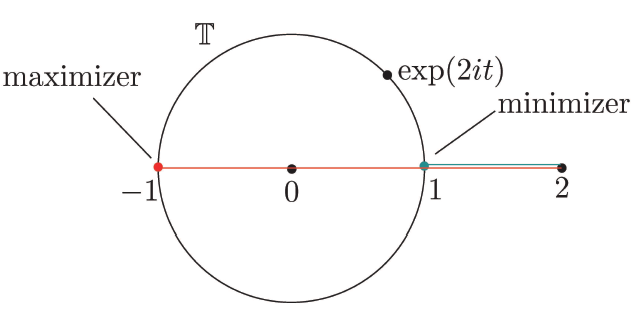
\includegraphics[width=0.4\textwidth]{./Solution/figs/fig-5-22}
\end{center}
\caption{단위원에서 $|z^2-2|$를 최대로 하는 점과 최소로 하는 점
}
\label{fig-5-22}
\end{figure}

\subsection*{연습문제 \ref{ex-4-29}}

$z\in \mathbb A_1 := \{ z\in\mathbb C\,:\, 0<|z-1|<1\}$에 대하여
\begin{align*}
\dfrac1{z(z-1)}
&= \dfrac1{(z-1+1)(z-1)} \\
&= \dfrac1{z-1}\Big(1-(z-1) + (z-1)^2 - (z-1)^3 + \cdots\Big) \\
&= \dfrac1{z-1} - 1 + (z-1) - (z-1)^2 + (z-1)^3 - \cdots.
\end{align*}

한편
$z\in \tilde {\mathbb A_1} := \{ z\in\mathbb C\,:\, 1<|z-1|\}$에 대하여
\begin{align*}
\dfrac1{z(z-1)}
&= \dfrac1{(z-1+1)(z-1)}
= \dfrac1{(z-1)^2\left( 1+ \dfrac1{z-1}\right)} \\
&= \dfrac1{(z-1)^2}\left( 1- \dfrac1{z-1} + \dfrac1{(z-1)^2} - \dfrac1{(z-1)^3} + \cdots \right) \\
&= \dfrac1{(z-1)^2} - \dfrac1{(z-1)^3} + \dfrac1{(z-1)^4} - \dfrac1{(z-1)^5} + \cdots.
\end{align*}

\subsection*{연습문제 \ref{ex-4-30}}

근의 분류 정리로부터 $z\in D$에서
$f(z) = (z-z_0)^mg(z)$이고 $g$는 복소해석함수로 $g(z_0)\ne0$이다.
$D$에서 $z_0$는 $f$의 유일한 근이므로, $D$에서 $g(z)\ne0$이다.
따라서 $1/g$가 복소해석함수이고 $z_0$를 중심으로 하는 원판에서 테일러 급수 전개가 가능하다.
즉, 상수 $R>0$이 존재하여
\[
\dfrac1{g(z)} = \sum_{n=0}^\infty c_n(z-z_0)^n,
\quad |z-z_0|<R
\]
이고 $c_0\ne0$이다 ($g(z_0)\ne0$이므로). 
$0<|z-z_0|<R$에 대하여,
\begin{align*}
\dfrac1{f(z)} 
&= \dfrac1{(z-z_0)^m g(z)} = \dfrac1{(z-z_0)^m} \sum_{n=0}^\infty c_n(z-z_0)^n \\
&= \dfrac{c_0}{(z-z_0)^m} +  \dfrac{c_1}{(z-z_0)^{m-1}} + \cdots 
+  \dfrac{c_{m-1}}{z-z_0} + \sum_{n=0}^\infty c_{m+n} (z-z_0)^n.
\end{align*}
따라서 $1/f$는 $z_0$에서 $m$ 중극을 갖는다.

\subsection*{연습문제 \ref{ex-4-31}}

$z\mapsto (z-z_0)^m f(z)$는 $D$에서 복소해석함수 $h$로 확장될 수 있다.
또한, 
\[
\neg\left( \lim_{z\to z_0} (z-z_0)^m f(z) = 0 \right)
\]
이므로 $h(z_0) \ne 0$이다. 
$z\in D$에서 $f(z)\ne0$이므로, 모든 $z\in D$에 대하여 $h(z)\ne0$이다.
따라서
\[
\dfrac1{f(z)} = \dfrac{(z-z_0)^m}{h(z)},
\quad z\in D\setminus \{z_0\}
\]
이고 
\[
g(z):= \dfrac{(z-z_0)^m}{h(z)},
\quad z\in D
\]
로 정의하면 $g$는 $D$에서 복소해석함수이다.
$\dfrac1{h(z_0)}\ne0$이므로 $z_0$는 $g$의 $m$ 중근이다.

\subsection*{연습문제 \ref{ex-4-32}}

모든 $n<-m$에 대하여 $c_n=0$이므로
\[
f(z) = \dfrac{c_{-m}}{(z-z_0)^m} + \dfrac{c_{-m+1}}{(z-z_0)^{m-1}}
+ \cdots + \dfrac{c_{-1}}{z-z_0} + \sum_{n=0}^\infty c_n(z-z_0)^n.
\]
따라서 $(z-z_0)^m f(z) = c_{-m} + c_{-m+1}(z-z_0) + \cdots + c_{-1}(z-z_0)^{m-1} + \cdots$는
\[
\Delta:= \{ z\in \mathbb C \,:\, |z-z_0|<R\}
\]
에서 복소해석함수 $g$로 확장가능하다.
$|z-z_0| <R$에서 
$g(z) = c_{-m} + c_{-m+1}(z-z_0) + \cdots + c_{-1}(z-z_0)^{m-1} + \cdots$의
테일러 정리를 적용하면,
\[
c_{-1} = \dfrac1{(m-1)!}\dfrac{d^{m-1}g}{dz^{m-1}}(z_0).
\]
한편, $g^{(m-1)}$은 $\Delta$에서 복소해석함수이며,
특히, $z_0$에서 연속이므로
\[
g^{(m-1)}(z_0) = \lim_{z\to z_0} g^{(m-1)}(z).
\]
또한, $0<|z-z_0|<R$에서 $g(z) = (z-z_0)^m f(z)$이고
$\Delta$의 점 $z\ne z_0$에서
\[
g^{(m-1)}(z) = \dfrac{d^{m-1}}{dz^{m-1}}((z-z_0)^m f(z)).
\]
따라서
\begin{align*}
c_{-1} &= \dfrac1{(m-1)!} g^{(m-1)}(z_0) 
= \dfrac1{(m-1)!} \lim_{z\to z_0} g^{(m-1)}(z) \\
&= \dfrac1{(m-1)!} \lim_{z\to z_0} \dfrac{d^{m-1}}{dz^{m-1}}((z-z_0)^m f(z)).
\end{align*}

\subsection*{연습문제 \ref{ex-4-33}}

\begin{itemize}
\item[(1)] 참. 
$c_{-1}=1\ne0$이고 $c_{-2} = c_{-3} = \cdots = 0$.
\item[(2)] 참.
\item[(3)] 참.
\item[(4)] 참.
\item[(5)] 참.
\end{itemize}

\subsection*{연습문제 \ref{ex-4-34}}

\begin{itemize}
\item[(1)]  $\sin z$는 $0$을 특이점으로 갖지 않는다.
$z\in \mathbb C$에 대하여
\[
\sin z = z - \dfrac{z^3}{3!} + \dfrac{z^5}{5!} - \cdots.
\]
\item[(2)] $\sin \dfrac1z$는 $0$을 본질적 특이점으로 갖는다. $z\ne0$에 대하여
\[
\sin \dfrac1z = \cdots + \dfrac1{5!z^5} - \dfrac1{3!z^3} + \dfrac1z.
\]
\item[(3)]  $\dfrac{\sin z}z$는 $0$에서 제거 가능한 특이점을 갖는다.
\[
\lim_{z\to 0} z\cdot \dfrac{\sin z}z = \lim_{z\to 0} \sin z = 0.
\]
따라서 $\dfrac{\sin z}{z} = 1  - \dfrac1{3!}z^2  + \dfrac1{5!}z^4 - \dfrac1{7!}z^6 + \cdots$
($z\ne0$).
\item[(4)] $\dfrac{\sin z}{z^2}$은 $0$에서 $1$차의 극을 갖는다.
$z\ne0$에 대하여
\[
\dfrac{\sin z}{z^2} = \dfrac1z - \dfrac z{3!} + \dfrac{z^3}{5!} - \dfrac{z^5}{7!} + \cdots.
\]
\item[(5)] $1/(\sin(1/z))$는 $0$에서 고립 특이점을 갖지 않는다. 왜냐하면,
$z_n = 1/(n\pi)$, $n\in\mathbb N$에서 
\[
\sin \dfrac1{z_n} = \sin(n\pi) = 0
\]
이고 $z_n = \dfrac1{n\pi} \stackrel{n\to\infty}{\longrightarrow} 0$
이기 때문이다. (이러한 현상은 예제 \ref{example-4-13}에서와 같다.)
\item[(6)] $z\sin\dfrac1z$는 $0$을 본질적 특이점으로 갖는다.
$z\ne0$에 대하여
\[
z\sin \dfrac1z = \cdots + \dfrac1{5!z^4} - \dfrac1{3!z^2} +1.
\]
\end{itemize}

\subsection*{연습문제 \ref{ex-4-35}}

\begin{itemize}
\item[(1)] 거짓.
$\Lim_{z\nearrow 0} |e^{\frac1x}| = \Lim_{x\nearrow 0} e^{\frac1x} = 0$
이므로 $\neg \left( \lim_{z\to 0} \left| \exp\dfrac1z\right| = + \infty \right)$.
\item[(2)] 참.
$0<|z-z_0|<R$에 대하여
\[
f(z) = \dfrac{c_{-m}}{(z-z_0)^m} + \dfrac{c_{-m+1}}{(z-z_0)^{m-1}} + \cdots 
+ \dfrac{c_{-1}}{z-z_0} + \sum_{n=0}^\infty c_n(z-z_0)^n
\]
을 만족하는 $R>0$이 존재하므로
\[
p:= c_{-m} + c_{-m+1}(z-z_0) + \cdots  + c_{-1}(z-z_0)^{m-1}
\]
이라 하면, $0<|z-z_0|<R$에서
\[
f(z) - \dfrac{p(z)}{(z-z_0)^m} = \sum_{n=0}^\infty c_n(z-z_0)^n.
\]
\item[(3)] 참.
$0$이 $f$의 $m$\,중근이라고 하자. ($f(0)\ne0$인 경우 $m=0$이라 하자.)
그러면 $f(z)=z^mg(z)$이고 $g(0)\ne0$인 복소해석함수 $g$가 존재한다.
$n>m$에 대하여, $z\ne0$이면
\[
\dfrac{f(z)}{z^n} = \dfrac{z^mg(z)}{z^n} = \dfrac{g(z)}{z^{n-m}}.
\]
따라서, $g(0)\ne0$이고 $n>m$이므로
\[
\lim_{z\to0} \left| \dfrac{f(z)}{z^n}\right| 
=\lim_{z\to0} \dfrac{|g(z)|}{|z|^{n-m}} = |g(0)|\cdot \lim_{z\to0}\dfrac1{|z|^{n-m}} = +\infty
\]
\item[(4)] 참.
뚫린 원판 $D=\{ z\in \mathbb C\,:\, 0<|z-z_0| <R\}$에서
$f,g$가 $0$이 아니고 $h_f(z_0)\ne0$, $h_g(z_0)\ne0$인 복소해석함수 $h_f, h_g$가 존재하여
모든 $z\in D$에 대하여
\[
\dfrac1{f(z)} = (z-z_0)^{m_f} h_f(z),\quad
\dfrac1{g(z)} = (z-z_0)^{m_g} h_g(z).
\]
따라서 $h_f(z_0)h_g(z_0)\ne0$이고 모든 $z\in D$에 대하여
\[
\dfrac1{f(z)g(z)} = (z-z_0)^{m_f+m_g} h_f(z)h_g(z).
\]
결론적으로, $fg$는 $z_0$에서 $m_f+m_g$차 극을 갖는다.
\end{itemize}

\subsection*{연습문제 \ref{ex-4-36}}

\[
f(z) = \exp \left(\dfrac 1z \right) + \exp \left(\dfrac1{1-z}\right),
\quad z\in \mathbb C\setminus\{0,1\}
\]
은 $\mathbb C\setminus\{0,1\}$에서 복소해석함수이다.
함수 $\exp(1/(1-z))$는 $z=0$ 근방에서 복소해석함수이고
$\exp(1/z)$는 $0$을 본질적 특이점으로 갖는다. 따라서 그 합 $f$는 $0$을
본질적 특이점으로 갖는다. (왜?) 한편, $1$ 근방에서 $\exp(1/z)$는 복소해석함수이고
$\exp(1/(1-z))$는 본질적 특이점을 갖는다. 따라서 $f$는 $z=1$도 본질적 특이점으로 갖는다.

\subsection*{연습문제 \ref{ex-4-37}}

$z_0$가 $g$의 고립 특이점이면 
$0<|z-z_0|<R$에서 로랑급수 전개
\[
g(z) = \sum_{n\in\mathbb Z} c_n(z-z_0)^n
\]
를 주는 적당한 $R>0$이 존재한다.
$c_n\ne0$인  $n<0$이 무한이 많으면 $z_0$는 $g$의 본질적 특이점이다.

그런데 주어진 $f$는 $|z|>1$로 주어진 뚫린 원판에서 로랑급수 전개
\[ 
z^{-1} + z^{-2} + z^{-3} + \cdots
\]
를 갖는다. 특이점 $0$의 특성을 규정하려면 
적당한 $R>0$에 대하여 $0<|z|<R$에서 함수를 살펴봐야 한다.
$|z|<1$에서는 로랑 급수가
\[
f(z) = - \dfrac1{1-z} = - (1+z+z^2+ z^3 + \cdots )
\]
이므로 $ |z|<1$에서 $f$는 복소해석함수이고
$z=0$에서 특이점을 갖지 않는다.

\subsection*{연습문제 \ref{ex-4-38}}

$z_0$가 $fg$의 고립 특이점임은 분명하다.
$f$와 $g$가 $z_0$에서 고립 특이점을 갖기 때문에
뚫린 원판 $0<|z-z_0|<R_f$에서 $f$가 복소해석함수인  $R_f>0$가 존재하고
뚫린 원판 $0<|z-z_0|<R_g$에서 $g$가 복소해석함수인  $R_g>0$가 존재한다.
따라서 뚫린 원판  $0<|z-z_0| < \min\{R_f, R_g\}$에서
$fg$는 복소해석함수이다.

$z_0$가 $fg$의 제거 가능한 특이점이거나 극이라고 가정하자.
그러면, 적당한 $m>1$이 존재하여
\[
\lim_{z\to z_0} (z-z_0)^m f(z)g(z) = 0
\]
을 만족한다.
$f$가 $z_0$에서 극을 가지므로, $m_f$차 극을 갖는다고 하면,
$f$는 $z_0$ 근방에서 $0$이 아니며, $0<|z-z_0|<R$에서
\[
f(z) = \dfrac{c_{-m_f}}{(z-z_0)^{m_f}} + \dfrac{c_{-m_f+1}}{(z-z_0)^{m_f-1}} +
\cdots + \dfrac{c_{-1}}{z-z_0} + \sum_{n=0}^\infty c_n(z-z_0)^n
\]
을 만족하는 $R>$이 존재한다.
여기서 $c _{-m_f} \ne0$이다.
따라서 $z\ne z_0$인 $z_0$ 근방에서
\begin{align*}
(z-z_0)^mg(z)
&= \dfrac1{(z-z_0)^{m_f}f(z)} \cdot \underbrace{(z-z_0)^{m_f}}_{\to0}
\underbrace{(z-z_0)^mf(z)g(z)}_{\to 0} \\
&\stackrel{z\to z_0}{\longrightarrow} \dfrac1{c_{-m_f}}\cdot 0 \cdot 0 - 0.
\end{align*}
그렇다면 $g$는 $z_0$에서 극을 갖거나 제거 가능한 특이점을 갖게 되고
가정에 모순이 되므로 $fg$는 $z_0$에서 본질적 특이점을 갖는다.

\subsection*{연습문제 \ref{ex-4-39}}

$\epsilon:= 1/n =:\delta(>0)$으로 설정하자.
카소라티-바이어스트라스 정리에 의해
$z_0$를 중심으로 반지름 $\delta$인 뚫린 원판에 점 $z_n$이 존재하여
$|f(z_n)-w|<\epsilon$을 만족한다.
즉, $|z_n - z_0| <1/n$이고 $|f(z_n) - w|< 1/n$.
따라서 $(z_n)_{n\in\mathbb N}$은 $z_0$로 수렴하고
$(f(z_n))_{n\in\mathbb N}$은 $w$로 수렴한다.

\subsection*{연습문제 \ref{ex-4-40}}

$1+\exp z =0$일 필요충분조건은 $ z\in \{ \pi i +2\pi n i \,:\, n\in \mathbb Z\}$이다.
따라서
\[
f(z):= \dfrac{\Log(z)}{1+\exp z}
\]
는 $(\mathbb C\setminus(-\infty,0])\setminus \{ \pi i +2\pi n i \,:\, n\in \mathbb Z\}$에서
복소해석함수이다.
$f$는 $\{ \pi i +2\pi n i \,:\, n\in \mathbb Z\}$에 속하는 점에서 $1$차의 극을 가진다.
경로 $\gamma$의 내부에는 $-\pi i$와  $3\pi i$가 속한다. 그림 \ref{fig-5-23}\을 참고하라.

\begin{figure}[h!]
\begin{center}
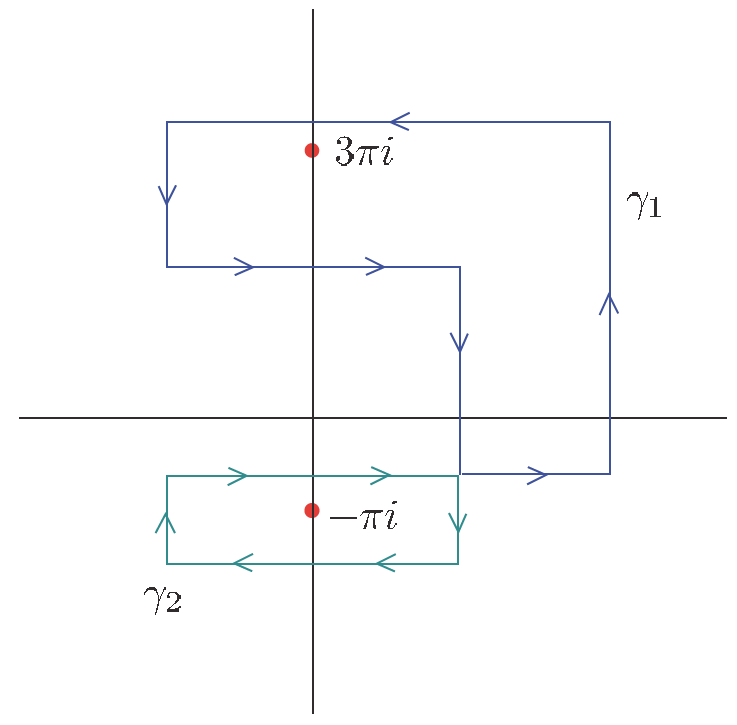
\includegraphics[width=0.5\textwidth]{./Solution/figs/fig-5-23}
\end{center}
\caption{닫힌경로 $\gamma_1$과 $\gamma_2$
}
\label{fig-5-23}
\end{figure}

\[
\int_\gamma f(z) dz = \int_{\gamma_1} f(z) dz + \int_{\gamma_2} f(z) dz
= 2\pi i (\res(f,3\pi i) - \res(f, -\pi i))
\]
이므로 $\res(f, 3\pi i)$와 $\res(f, \pi i)$를 계산해야 한다.
\[
\dfrac{\Log(z)}{1+\exp z} = \dfrac{c_{-1,3\pi i}}{z-3\pi i} + h_{3\pi i}
\]
로 쓸 수 있다. 여기서, $h_{3\pi i}$는 $3\pi i$ 근방에서 복소해석함수이다.
따라서
\begin{align*}
c_{-1,3\pi i}
&= \lim_{z\to 3\pi i} \dfrac{(z-3\pi i)\Log(z)}{1+\exp z} 
= \lim_{z\to 3\pi i} \dfrac{z-3\pi i}{\exp z - \exp(3\pi i)}\cdot \Log(z) \\
&= \dfrac1{\exp z|_{z=3\pi i}} \cdot \Log(3\pi i) = -1\left( \log|3\pi i| + i\dfrac\pi2 \right) \\
&= - \log 3 - \log\pi- i\dfrac\pi2.
\end{align*}
한편,
\[
\dfrac{\Log(z)}{1+\exp z} = \dfrac{c_{-1,-\pi i}}{z-(-\pi i)} + h_{-\pi i}
\]
로 쓸 수 있다. 여기서, $h_{-\pi i}$는 $-\pi i$ 근방에서 복소해석함수이다.
따라서
\begin{align*}
c_{-1,-\pi i}
&= \lim_{z\to -\pi i} \dfrac{(z-(-\pi i))\Log(z)}{1+\exp z} 
= \lim_{z\to -\pi i} \dfrac{z-(-\pi i)}{\exp z - \exp(-\pi i)}\cdot \Log(z) \\
&= \dfrac1{\exp z|_{z=-\pi i}} \cdot \Log(-\pi i) 
= -1\left( \log|-\pi i| + i\left(-\dfrac\pi2 \right)\right) \\
&= - \log\pi +  i\dfrac\pi2.
\end{align*}

종합하면,
\[
\int_\gamma \dfrac{\Log(z)}{1+\exp z} dz
= 2\pi i \left( -\log 3 - \log \pi - i\dfrac\pi2 + \log \pi - i\dfrac\pi 2\right)
= 2\pi^2 - (2\pi \log 3)i.
\]

\subsection*{연습문제 \ref{ex-4-41}}

$\gamma(\theta)  = \exp(i\theta)$, $\theta\in [0,2\pi)$의
원형경로로 적분경로 $\gamma$를 정의하자.
그러면,
\begin{align*}
\int_0^{2\pi} \dfrac{\cos\theta}{5+4\cos\theta} d\theta
&= \int_\gamma \dfrac{\dfrac{z+\frac1z}2}{5+4\dfrac{z+\frac1z}2}\cdot \dfrac1{iz}dz
= \int_\gamma \dfrac{z^2+1}{2iz(2z^2+5z+1)}dz \\
&= \int_\gamma \dfrac{z^2+1}{2iz(2z+1)(z+2)}dz.
\end{align*}
\[
f(z):= \dfrac{z^2+1}{2iz(2z+1)(z+2)}
\]
라 정의하면, $f$는 $0$, $-1/2$, $-2$에서 $1$차의 극을 갖는다.
경로 $\gamma$의 내부에는 $0$과 $-1/2$이 있으므로
유수정리를 쓰면,
\begin{align*}
\int_0^{2\pi} & \dfrac{\cos\theta}{5+4\cos\theta} d\theta \\
&=2\pi i \left(\res(f,0) + \res(f,-1/2)\right) \\
&=2\pi i \left(\lim_{z\to0} \dfrac{z\cdot(z^2+1)}{2iz(2z+1)(z+2)}
+ \lim_{z\to1/2} \dfrac{(z+1/2)\cdot(z^2+1)}{2iz(2z+1)(z+2)} \right) \\
&= 2\pi i \left( \dfrac1{2i\cdot 1\cdot 2} 
+ \dfrac{1\cdot\frac54}{2i\cdot (-\frac12)\cdot2\cdot\frac32} \right)
= 2\pi i \left( \dfrac1{4i} - \dfrac5{12i} \right) \\
&= -\dfrac\pi3.
\end{align*}

\subsection*{연습문제 \ref{ex-4-42}}

\begin{itemize}
\item[(1)] $f_1$을 다음과 같이 정의하자.
\[
f_1(z) = \dfrac1{1+z^2}.
\]
그러면 $f_1$은 $i$와 $-i$에서 $1$차 극을 갖는다. 따라서
\begin{align*}
\int_0^\infty \dfrac1{1+x^2}dx &= \dfrac12 \cdot2\pi i \cdot \res(f_1, i)
= \pi i \cdot \lim_{z\to i} \dfrac{z-i}{1+z^2} \\
&= \pi i \cdot \lim_{z\to i} \dfrac1{z+i} = \pi i \cdot \dfrac1{2i} = \dfrac\pi 2.
\end{align*}
\item[(2)] $f_2$를 다음과 같이 정의하자.
\[
f_2(z) = \dfrac1{(a^2+z^2)(b^2+z^2)}.
\]
그러면 $f_2$는 $ai$, $-ai$, $bi$, $-bi$에서 $1$차 극을 갖는다. 
$f_2$가 우함수이므로
\begin{align*}
\int_0^\infty \dfrac1{(a^2+x^2)(b^2+x^2)}dx
&= \dfrac12 \cdot 2\pi i \left( \res(f_2, ai) + \res(f_2, bi) \right) \\
&= \pi i \left( \dfrac1{(b^2-a^2)2ai} + \dfrac1{(a^2-b^2)2bi} \right) \\
&= \dfrac\pi{2(a^2-b^2)} \left( \dfrac1b-\dfrac1a\right) = \dfrac\pi{2ab(a+b)}.
\end{align*}
\item[(3)]  $f_3$를 다음과 같이 정의하자.
\[
f_3(z) = \dfrac1{(1+z^2)^2}.
\]
그러면 $f_3$는 $i$, $-i$에서 $2$차 극을 갖는다. 
\begin{align*}
\int_0^\infty \dfrac1{(1+x^2)^2}dx
&= \dfrac12 \cdot 2\pi i \cdot \res(f_3, i) \\
&= \dfrac\pi{1!}\cdot \lim_{z\to i} \dfrac d{dz} \left(
(z-i)^2 \cdot \dfrac1{(z-i)^2(z+i)^2} \right) \\
&= \pi i \cdot \lim_{z\to i} \dfrac{-2}{(z+i)^3} = \pi i \cdot \dfrac{-2}{-8i}
= \dfrac\pi4.
\end{align*}
\item[(4)] $f_4$를 다음과 같이 정의하자.
\[
f_4(z) = \dfrac{1+z^2}{1+z^4}.
\]
그러면 $f_4$는 다음 점들에서 $1$차 극을 갖는다. 
\[
p_1 =\exp\left(\dfrac{\pi i }4\right), \quad
p_2 =\exp\left(\dfrac{3\pi i }4\right), \quad
p_3 =\exp\left(\dfrac{5\pi i }4\right), \quad
p_4 =\exp\left(\dfrac{7\pi i }4\right).
\]
\begin{align*}
\int_0^\infty \dfrac{1+x^2}{1+x^4}dx 
&= \dfrac12\cdot 2\pi  i\left(\res(f_4,p_1) + \res(f_4,p_2) \right)
=\pi i \left( \dfrac{1+p_1^2}{4p_1^3} + \dfrac{1+p_2^2}{4p_2^3} \right) \\
&= \pi i \left( \dfrac{p_1}{4p_1^4} + \dfrac1{4p_1} + \dfrac{p_2}{4p_2^4} + \dfrac1{4p_2} \right)
= \pi i \left( - \dfrac{p_1+p_2}{4} + \dfrac1{4p_1} + \dfrac1{4p_2} \right) \\
&= \pi i \left( - \dfrac{\exp(i\pi/4) - \exp(-\pi i/4)}4 
+ \dfrac{\exp(-i\pi/4) - \exp(i\pi/4)}4 \right) \\
&= \pi i \left( - \dfrac{i\sin(\pi/4)}2 + \dfrac{-i\sin(\pi/4)}2 \right)
= \pi i \cdot(-i) \cdot \dfrac1{\sqrt{2}} = \dfrac\pi{\sqrt{2}}.
\end{align*}
\end{itemize}
 
\subsection*{연습문제 \ref{ex-4-43}}

유수정리를 이용하면,
\begin{align*}
\int_C \dfrac{\exp z}{z^{n+1}} dz
&= 2\pi i \cdot \res\left(\dfrac{\exp z}{z^{n+1}}, 0\right) 
= \dfrac{2\pi i}{n!} \cdot \lim_{z\to 0} \dfrac{d^n}{dz^n} 
\left(z^{n+1}\cdot \dfrac{\exp z}{z^{n+1}} \right) \\
&= \dfrac{2\pi i}{n!} \cdot \lim_{z\to 0} \dfrac{d^n}{dz^n} \exp z
= \dfrac{2\pi i}{n!} \cdot \lim_{z\to 0} \exp z 
= \dfrac{2\pi i}{n!} \cdot \exp 0 \\
&= \dfrac{2\pi i}{n!} \cdot 1 =  \dfrac{2\pi i}{n!}.
\end{align*}
따라서,
\begin{align*}
\dfrac{2\pi i}{n!}
&= \int_0^{2\pi} \dfrac{\exp(\cos\theta + i \sin\theta)}
{\cos((n+1)\theta) + i\sin((n+1)\theta)} \cdot
i(\cos\theta + i\sin\theta) d\theta \\
&= i\int_0^{2\pi} \exp(\cos\theta + i\sin\theta)\cdot
\left(\cos(n\theta) - i\sin(n\theta) \right) d\theta \\
&=i\int_0^{2\pi} \exp(\cos\theta)\left(\cos(n\theta-\sin\theta)
- i \sin(n\theta - \sin\theta)\right)d\theta.
\end{align*}
양변의 허수부를 비교하여
\[
\int_0^{2\pi} \exp(\cos\theta)\cdot \cos(n\theta-\sin\theta) d\theta
= \dfrac{2\pi}{n!}.
\]
 
\subsection*{연습문제 \ref{ex-4-44}}

중심이 $z_0$인 작은 뚫린 원판 $D$에서 $f(z)\ne0$이고
\begin{equation}\label{eq-5-26}
f(z) = (z-z_0)h(z)
\end{equation}
를 만족하는 $h(z_0)\ne0$인 복소해석함수 $h$가 존재한다.
식 \eqref{eq-5-26}에 의해
$f'(z) = h(z) + (z-z_0)h'(z)$로 쓸 수 있다.
특히, $f'(z_0) = h(z_0)$이다.
$z\in D\setminus \{z_0\}$에 대하여
\[
\dfrac1{f(z)} = \dfrac1{(z-z_0)h(z)}
\]
이고 $\dfrac1h$이 $D$에서 복소해석함수이므로
\[
\dfrac1{h(z)} = d_0 + d_1(z-z_0) + \cdots
\]
이고 $d_0 = \dfrac1{h(z_0)} = \dfrac1{f'(z_0)}$이다.
따라서 $z\in D\setminus\{z_0\}$에 대하여
\[
\dfrac1{f(z_0)} = \dfrac1{z-z_0} \cdot(d_0 + d_1(z-z_0) + \cdots)
= \dfrac{d_0}{z-z_0} + d_1 + d_2(z-z_0) + \cdots
\]
이고 $\res\left( \dfrac1f, z_0\right) = d_0 = \dfrac1{f'(z_0)}$를 
얻는다\footnote{
역주: 이 연습문제는 예제 \ref{example-4-19}에서 사용한 계산 기법을 일반화한 것이다.
유사한 방법이 연습문제 \ref{ex-4-42}에서도 사용되었다.
이 결과를 기억해두면 분모의 차수가 큰 유리함수의 유수 계산에 유용하다.
}.

\subsection*{연습문제 \ref{ex-4-45}}

$f(z) = \sin z$라고 하자.
$f$는 $k\pi$, $k\in\mathbb Z$에서 $1$차의 근을 갖는다.
앞의 연습문제에 의하여
\[
\res\left(\dfrac1{\sin z}, k\pi \right)
= \dfrac1{\sin' z|_{z=k\pi}} = \dfrac1{\cos(k\pi)}
= \dfrac1{(-1)^k} = (-1)^k.
\]

\subsection*{연습문제 \ref{ex-4-46}}

\begin{itemize}
\item[(1)]  $f_0=1\le 2^0=1$, $f_1 = 1\le 2^1=2$이고,
어떤 $n\ge1$이 존재하여 모든 $m\le n$에 대하여
$f_m\le 2^m$이 성립한다고 가정하면,
\[
f_{n+1} = f_n + f_{n-1} \le 2^n + 2^{n-1}
= 2^{n-1} \cdot3 < 2^{n-1}\cdot 4 = 2^{n+1}.
\]
따라서 $n+1$에서도 성립한다.

\item[(2)] $|z|<1/2$이면, 모든 $n\in \mathbb N$에 대하여
$\sqrt[n]{|c_nz^n|} = \sqrt[n]{|c_n|}\cdot|z| \le \sqrt[n]{2^n}\cdot|z| = 2|z| < 1$.
근판정법에 의해
\[
\sum_{n=0}^\infty |c_nz^n|
\]
은 $|z|<1/2$일 때 수렴한다. 따라서 $F$의 수렴 반지름은 $1/2$보다 크거나 같다.

\item[(3)] $|z|<1/2$에 대하여
\begin{align*}
zF(z) &= f_0z + f_1z^2 + f_2z^3 + \cdots, \\
z^2F(z) &= \phantom{f_0z+\ }\, f_0z^2 + f_1z^3 + \cdots.
\end{align*}
두 식을 더하면,
\begin{align*}
zF(z) + z^2F(z) &= 1\cdot z + (f_1+f_0)z^2 + (f_2+f_1)z^3 + \cdots\\
&= f_1z + f_2z^2 + f_3z^3 + \cdots \\
&= (f_0 +  f_1z + f_2z^2 + f_3z^3 + \cdots ) - f_0 \\
&= F(z) -1.
\end{align*}
따라서
\[
1 = F(z) - zF(z) -z^2F(z) = (1-z-z^2)F(z)
\]
이므로,
$|z|<\dfrac12$에서 $F(z) = \dfrac1{1-z-z^2}$.

\item[(4)] 
\begin{align}
\dfrac1{z^{n+1}(1-z-z^2)}
&= \dfrac{F(z)}{z^{n+1}} \nonumber \\ 
&= \dfrac{f_0+\cdots + f_{n-1}z^{n-1} + f_nz^n + f_{n+1}z^{n+1} + \cdots}{z^{n+1}} \nonumber \\
&= \dfrac{f_0}{z^{n+1}} + \dfrac{f_1}{z^n} + \cdots + \dfrac{f_n}{z} + f_{n+1} + f_{n+2}z + \cdots
\label{eq-5-27}
\end{align}
이므로  유수를 계산하면
\[
\res\left( \dfrac1{z^{n+1}(1-z-z^2)}, 0\right)
= f_n. \ (\text{식 \eqref{eq-5-27}에서 $\dfrac1z$의 계수})
\]

\item[(5)] $|z|=R>2$에 대하여
\begin{align*}
|1-z-z^2| &\ge |z^2+z| -1 = |z|\cdot|z+1| -1 = R\cdot |z+1| -1 \\
&\ge R\cdot(|z|-1)-1 = R\cdot(R-1) -1 = R^2 -R -1 \\
&>0 \ \text{($R>2$이므로)}.
\end{align*}
$C_R:[0,2\pi] \to \mathbb C$가 다음과 같은 원형경로이면,
\[
C_R(t) = R\exp(it), \quad t\in[0,2\pi],
\]
\begin{align*}
\left| \int_{C_R} \dfrac1{z^{n+1}(1-z-z^2)} dz \right|
&\le \dfrac1{R^{n+1}}\cdot\dfrac1{R^2-R-1}\cdot 2\pi R\\
&= \dfrac1{R^n}\cdot\dfrac{2\pi}{R^2-R-1}
\xrightarrow{R\to\infty} 0.
\end{align*}
$G(z):= \dfrac1{z^{n+1}(1-z-z^2)} $라 정의하면, $G$는
\begin{itemize}
\item[(a)] $0$에서 $n+1$차 극을 갖는다.
\item[(b)] $\dfrac{-1+\sqrt{5}}2$에서 $1$차 극을 갖는다.
\item[(c)] $\dfrac{-1-\sqrt{5}}2$에서 $1$차 극을 갖는다.
\end{itemize}
따라서 $R>2$에 대하여,
\[
\res(G,0) + \res\left(G, \dfrac{-1+\sqrt{5}}2\right)
+ \res\left(G, \dfrac{-1-\sqrt{5}}2\right) 
= \dfrac1{2\pi i} \int_{C_R} G(z) dz.
\]
\begin{align*}
\res(G,0) &+ \res\left(G, \dfrac{-1+\sqrt{5}}2\right)
+ \res\left(G, \dfrac{-1-\sqrt{5}}2\right) \\
&=  \lim_{R\to\infty} \dfrac1{2\pi i} \int_{C_R} G(z) dz = 0
\end{align*}
이므로,
\[
f_n = -\res\left(G, \dfrac{-1+\sqrt{5}}2\right)
- \res\left(G, \dfrac{-1-\sqrt{5}}2\right).
\]
\begin{align*}
\res\left(G, \dfrac{-1+\sqrt{5}}2\right)
&= \lim_{z\to \frac{-1+\sqrt{5}}2} \left( z - \dfrac{-1+\sqrt{5}}2 \right)
\cdot \dfrac1{z^{n+1}(1-z-z^2)} \\
&= \dfrac1{\left(\dfrac{-1+\sqrt{5}}2\right)^{n+1} \cdot(-\sqrt{5})} \\
&= \left(\dfrac{1+\sqrt{5}}2\right)^{n+1} \left(- \dfrac1{\sqrt{5}} \right).
\end{align*}
\[
\res\left(G, \dfrac{-1-\sqrt{5}}2\right)
= \dfrac1{\left(\dfrac{-1-\sqrt{5}}2\right)^{n+1} \cdot(\sqrt{5})} 
= \left(\dfrac{1-\sqrt{5}}2\right)^{n+1} \left( \dfrac1{\sqrt{5}} \right).
\]
이를 종합하면,
\begin{align*}
f_n &= \dfrac1{\sqrt{5}} \cdot \left(\dfrac{1+\sqrt{5}}2\right)^{n+1}
- \dfrac1{\sqrt{5}} \cdot \left(\dfrac{1-\sqrt{5}}2\right)^{n+1} \\
&= \dfrac1{\sqrt{5}} \cdot \left( \left(\dfrac{1+\sqrt{5}}2\right)^{n+1}
- \left(\dfrac{1-\sqrt{5}}2\right)^{n+1} \right).
\end{align*}



\end{itemize}












